El dissenyador d'una casa de perfums ha decidit que l'ampolla del proper perfum que l'empresa traurà al mercat
serà de vidre i tindrà la forma d'un cilindre amb una mitja esfera a la part superior, tal com es pot veure a
la figura següent:
\begin{center}
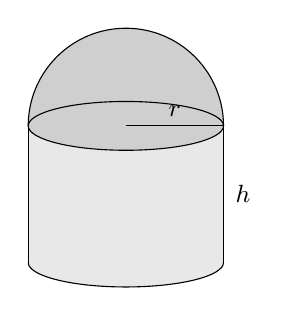
\begin{tikzpicture}[scale=0.62]
  \fill[gray!18] (-2,0) -- (-2,-2.8) arc[start angle=180,end angle=360,x radius=2,y radius=0.5] -- (2,0) -- cycle;
  \fill[gray!38] (2,0) arc[start angle=0,end angle=180,radius=2]
    arc[start angle=180,end angle=360,x radius=2,y radius=0.5];
  \draw (-2,0) arc[start angle=180,end angle=0,radius=2];
  \draw (0,0) ellipse [x radius=2,y radius=0.5];
  \draw (-2,0) -- (-2,-2.8);
  \draw (2,0) -- (2,-2.8);
  \draw (-2,-2.8) arc[start angle=180,end angle=360,x radius=2,y radius=0.5];
  \draw (0,0) -- (2,0);
  \node[above,font=\small] at (1,0) {$r$};
  \node[right,font=\small] at (2.05,-1.4) {$h$};
\end{tikzpicture}
\end{center}
El perfum estarà contingut a la part cilíndrica, la qual té una capacitat de $100\ \text{cm}^3$. L'enginyer a
càrrec del procés de producció es proposa minimitzar el cost total del vidre usat i, per tant, vol que la
superfície total de l'ampolla sigui mínima.

\emph{Nota:} Recordeu que la superfície d'una esfera ve donada per la fórmula $4\pi r^2$, on
$r$ és el radi.

\begin{apartats}

\apartat{1}
Comproveu que la superfície total de l'ampolla de perfum ve donada per la fórmula $S(r)=3\pi r^2+\dfrac{200}{r}$.

\begin{solucio}
Com que el volum de la part cilíndrica ha de ser de $100\ \text{cm}^3$, tenim que $\pi r^2h=100$ i, per tant,
$h=\frac{100}{\pi r^2}$. La superfície total de l'ampolla s'obté sumant la superfície de la base, $\pi r^2$, la
superfície lateral del cilindre, $2\pi rh$, i la superfície de la mitja esfera superior,
$\frac12\,4\pi r^2=2\pi r^2$; per tant, és
\[
S=\pi r^2+2\pi rh+2\pi r^2=3\pi r^2+2\pi rh .
\]
Si substituïm $h$ per l'expressió que tenim en funció de $r$, obtenim la funció
\[
S(r)=3\pi r^2+2\pi r\cdot\frac{100}{\pi r^2}=3\pi r^2+\frac{200}{r}.
\]

\textit{Pauta oficial:} 0,5 per la lligadura donada pel volum i 0,5 pel càlcul correcte de la fórmula de
l'àrea total.
\end{solucio}

\apartat{1,5}
Quines dimensions ha de tenir l'ampolla de perfum perquè la superfície total sigui mínima? Quina és la
superfície total de l'ampolla en aquest cas?

\begin{solucio}
Busquem ara el mínim d'aquesta funció calculant-ne la derivada: $S'(r)=6\pi r-\dfrac{200}{r^2}$. Igualant-la a
zero, $S'(r)=0$, obtenim
\[
6\pi r-\frac{200}{r^2}=0\;\rightarrow\;6\pi r=\frac{200}{r^2}\;\rightarrow\;r^3=\frac{100}{3\pi}\;\rightarrow\;
r=\sqrt[3]{\frac{100}{3\pi}}\simeq2{,}2\ \text{cm}.
\]
Per verificar que es tracta d'un mínim, podem utilitzar la segona derivada, $S''(r)=6\pi+\dfrac{400}{r^3}$, que
és clarament positiva per a qualsevol $r$ positiu. Per tant, per a $r=2{,}2$ cm l'ampolla té superfície total
mínima. En aquest cas tenim $h=\frac{100}{\pi\cdot2{,}2^2}=6{,}6$ cm, i la superfície total mínima és de
$S(2{,}2)=3\pi\cdot2{,}2^2+2\pi\cdot2{,}2\cdot6{,}6\simeq136{,}8\ \text{cm}^2$.

\textit{Pauta oficial:} 0,5 pel càlcul de la derivada, 0,25 per trobar el valor de $r$, 0,25 per comprovar que
es tracta d'un mínim, i 0,5 per donar la resposta completa (dimensions i àrea total).

\textit{Nota del banc:} el criteri calcula la superfície amb $r$ i $h$ ja arrodonits. Amb els valors exactes,
a l'òptim és $h=3r$ (perquè $\pi r^2h=100=3\pi r^3$), i la superfície mínima és
$S=9\pi r^2\approx136{,}5\ \text{cm}^2$. Una resposta amb aquest valor també és correcta.
\end{solucio}

\end{apartats}
